\documentclass[11pt,a4paper]{article}

% Packages
\usepackage[utf8]{inputenc}
\usepackage[margin=1in]{geometry}
\usepackage{graphicx}
\usepackage{hyperref}
\usepackage{amsmath}
\usepackage{amssymb}
\usepackage{listings}
\usepackage{xcolor}
\usepackage{tikz}
\usepackage{pgfplots}
\usepackage{array}
\usepackage{booktabs}
\usepackage{longtable}
\usepackage{fancyhdr}
\usepackage{tcolorbox}
\usepackage{enumitem}
\usepackage{float}

% TikZ libraries
\usetikzlibrary{shapes,arrows,positioning,fit,backgrounds,calc,shadows}
\pgfplotsset{compat=1.18}

% Color definitions
\definecolor{codegreen}{rgb}{0,0.6,0}
\definecolor{codegray}{rgb}{0.5,0.5,0.5}
\definecolor{codepurple}{rgb}{0.58,0,0.82}
\definecolor{backcolour}{rgb}{0.95,0.95,0.92}
\definecolor{emergencyred}{rgb}{0.8,0.1,0.1}
\definecolor{highyellow}{rgb}{1,0.8,0}
\definecolor{mediumblue}{rgb}{0.2,0.4,0.8}
\definecolor{lowgreen}{rgb}{0.2,0.6,0.2}

% Code listing style
\lstdefinestyle{mystyle}{
    backgroundcolor=\color{backcolour},   
    commentstyle=\color{codegreen},
    keywordstyle=\color{magenta},
    numberstyle=\tiny\color{codegray},
    stringstyle=\color{codepurple},
    basicstyle=\ttfamily\footnotesize,
    breakatwhitespace=false,         
    breaklines=true,                 
    captionpos=b,                    
    keepspaces=true,                 
    numbers=left,                    
    numbersep=5pt,                  
    showspaces=false,                
    showstringspaces=false,
    showtabs=false,                  
    tabsize=2
}
\lstset{style=mystyle}

% Header and footer
\pagestyle{fancy}
\fancyhf{}
\fancyhead[L]{RentMatrix AI Maintenance System}
\fancyhead[R]{Technical Architecture v1.0}
\fancyfoot[C]{\thepage}



\begin{document}


\thispagestyle{empty}



% ============================================================================
% EXECUTIVE SUMMARY
% ============================================================================

% ============================================================================
% ARCHITECTURE OVERVIEW
% ============================================================================
\section{High-Level System Architecture}

\subsection{System Components}

The RentMatrix AI system consists of seven major layers:

\begin{enumerate}
    \item \textbf{Input Layer}: Receives maintenance requests from tenants
    \item \textbf{Preprocessing Layer}: Validates, normalizes, and extracts metadata
    \item \textbf{Safety Net Layer}: Rule-based emergency detection (hard overrides)
    \item \textbf{Context Enrichment Layer}: Gathers contextual intelligence (weather, history, etc.)
    \item \textbf{AI Agent Orchestration Layer}: Five specialized LLM agents
    \item \textbf{Routing Layer}: Confidence-based decision routing
    \item \textbf{PM Dashboard Layer}: Human-in-the-loop review interface
\end{enumerate}

\subsection{System Flow Diagram}

\begin{figure}[H]
\centering
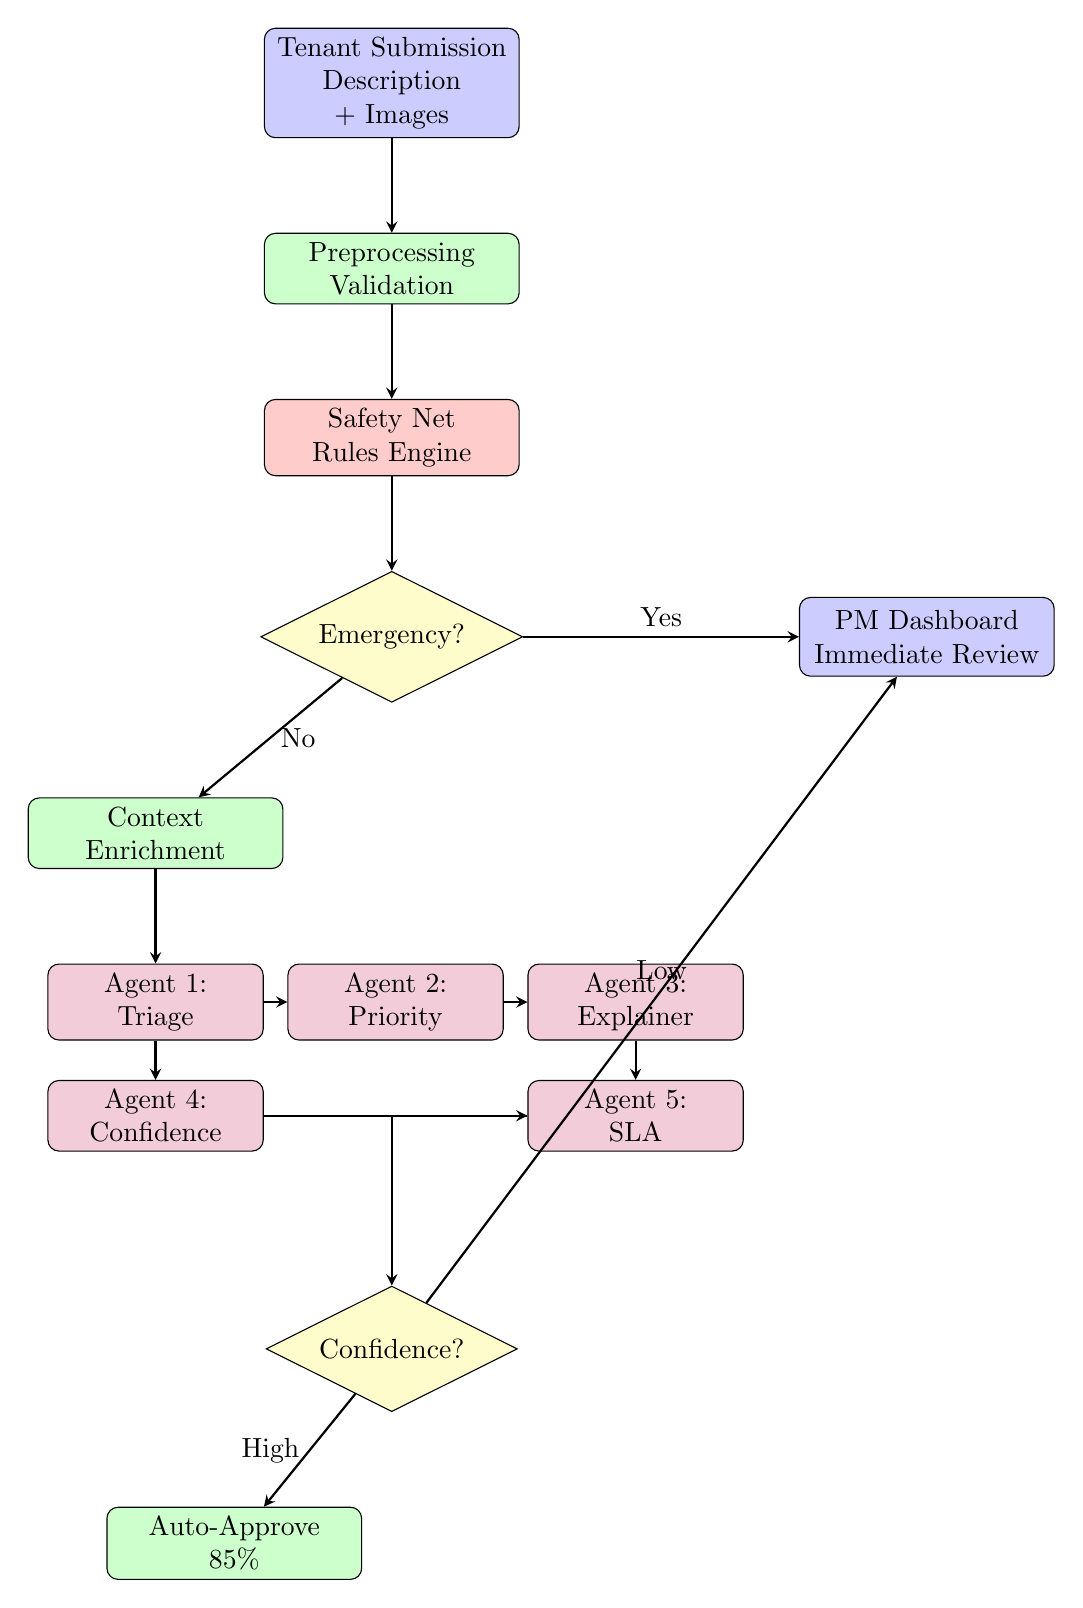
\begin{tikzpicture}[
    node distance=1.2cm and 1.5cm,
    box/.style={rectangle, draw, fill=blue!20, text width=3cm, align=center, rounded corners, minimum height=1cm},
    decision/.style={diamond, draw, fill=yellow!20, text width=2cm, align=center, aspect=2},
    process/.style={rectangle, draw, fill=green!20, text width=3cm, align=center, rounded corners, minimum height=0.8cm},
    safety/.style={rectangle, draw, fill=red!20, text width=3cm, align=center, rounded corners, minimum height=0.8cm},
    agent/.style={rectangle, draw, fill=purple!20, text width=2.5cm, align=center, rounded corners, minimum height=0.7cm},
    arrow/.style={->, >=stealth, thick}
]

% Input
\node[box] (input) {Tenant Submission\\Description + Images};

% Preprocessing
\node[process, below=of input] (preprocess) {Preprocessing\\Validation};

% Safety Net
\node[safety, below=of preprocess] (safety) {Safety Net\\Rules Engine};

% Decision
\node[decision, below=of safety] (emergency) {Emergency?};

% Context Enrichment
\node[process, below=of emergency, xshift=-3cm] (context) {Context\\Enrichment};

% Agents (arranged horizontally)
\node[agent, below=of context] (agent1) {Agent 1:\\Triage};
\node[agent, right=0.3cm of agent1] (agent2) {Agent 2:\\Priority};
\node[agent, right=0.3cm of agent2] (agent3) {Agent 3:\\Explainer};
\node[agent, below=0.5cm of agent1] (agent4) {Agent 4:\\Confidence};
\node[agent, below=0.5cm of agent3] (agent5) {Agent 5:\\SLA};

% Routing
\node[decision, below=of agent4, xshift=3cm, yshift=-0.5cm] (routing) {Confidence?};

% PM Dashboard
\node[box, right=of emergency, xshift=2cm] (pm) {PM Dashboard\\Immediate Review};

% Auto-approve
\node[process, below=of routing, xshift=-2cm] (auto) {Auto-Approve\\85\%};

% Arrows
\draw[arrow] (input) -- (preprocess);
\draw[arrow] (preprocess) -- (safety);
\draw[arrow] (safety) -- (emergency);
\draw[arrow] (emergency) -- node[right] {No} (context);
\draw[arrow] (emergency) -- node[above] {Yes} (pm);
\draw[arrow] (context) -- (agent1);
\draw[arrow] (agent1) -- (agent2);
\draw[arrow] (agent2) -- (agent3);
\draw[arrow] (agent1) -- (agent4);
\draw[arrow] (agent3) -- (agent5);
\draw[arrow] (agent4) -- (agent5);
\draw[arrow] (agent5) -| (routing);
\draw[arrow] (routing) -- node[left] {High} (auto);
\draw[arrow] (routing) -- node[above] {Low} (pm);

\end{tikzpicture}
\caption{High-Level System Flow}
\end{figure}

 

\subsection{Multi-Agent Architecture}

The system employs five specialized AI agents, each with a specific responsibility:

\begin{table}[H]
\centering
\small
\begin{tabular}{p{2.5cm}p{3.5cm}p{3cm}p{2.5cm}}
\toprule
\textbf{Agent} & \textbf{Purpose} & \textbf{Model} & \textbf{Output} \\
\midrule
1. Triage Classifier & Classify severity \& trade & GPT-5 (multimodal) & Severity, Trade, Confidence \\
\midrule
2. Priority Calculator & Calculate urgency score (0-100) & GPT-5-mini & Priority Score, Modifiers \\
\midrule
3. Explainer & Generate PM justification & GPT-5 & Human-readable explanation \\
\midrule
4. Confidence Evaluator & Self-assess quality & GPT-5 & Confidence (0.0-1.0) \\
\midrule
5. SLA Mapper & Map score to deadlines & Deterministic & Response/Resolution times \\
\bottomrule
\end{tabular}
\caption{AI Agent Specifications}
\end{table}






% ============================================================================
% DETAILED ARCHITECTURE
% ============================================================================
\section{Detailed System Architecture}

\subsection{Layer 1: Input Processing}

\subsubsection{Input Schema}

\begin{lstlisting}[language=Python, caption=Maintenance Request Input Schema]
class MaintenanceRequest:
    # Core fields (required)
    tenant_id: UUID
    property_id: UUID
    unit_id: UUID
    description: str  # Free text, 10-2000 chars
    category: Enum[PLUMBING, ELECTRICAL, HVAC, 
                   APPLIANCE, GENERAL, OTHER]
    
    # Optional fields
    severity_hint: Optional[str]  # Tenant's perception
    images: List[ImageFile]  # 0-5 images, max 10MB each
    reported_at: datetime
    
    # Auto-populated
    request_id: UUID
    channel: Enum[WEB, MOBILE, SMS, EMAIL]
\end{lstlisting}

\subsubsection{Validation Rules}

\begin{table}[H]
\centering
\begin{tabular}{lp{8cm}}
\toprule
\textbf{Field} & \textbf{Validation Rule} \\
\midrule
description & 10-2000 characters, alphanumeric + punctuation \\
images & Format: JPEG/PNG, Size: <10MB each, Count: 0-5 \\
category & Must be valid enum value \\
reported\_at & Must be within last 7 days (reject stale requests) \\
tenant\_id & Must exist in tenant database \\
\bottomrule
\end{tabular}
\caption{Input Validation Rules}
\end{table}

\subsection{Layer 2: Preprocessing}

\begin{lstlisting}[language=Python, caption=Preprocessing Pipeline (Pseudocode)]
def preprocess_request(request):
    """
    Preprocessing pipeline
    """
    # Step 1: Text normalization
    description = normalize_text(request.description)
    description = remove_pii(description)  # Strip names, addresses
    
    # Step 2: Image processing
    if request.images:
        images = []
        for img in request.images:
            # Compress to <2MB
            compressed = compress_image(img, target_size_mb=2)
            # Convert to base64
            base64_img = encode_base64(compressed)
            images.append(base64_img)
    
    # Step 3: Duplicate detection (5-min cache window)
    cache_key = hash(tenant_id + description + images_hash)
    if cached_result := redis.get(cache_key):
        return cached_result  # Cache hit (~5% of requests)
    
    # Step 4: Extract metadata
    metadata = extract_metadata(request)
    
    return ProcessedRequest(
        description=description,
        images=images,
        metadata=metadata
    )
\end{lstlisting}

 

\subsection{Layer 3: Safety Net (Rules Engine)}

\subsubsection{Emergency Keyword Detection}

\begin{tcolorbox}[colback=red!5!white,colframe=red!75!black,title=CRITICAL: 100\% Emergency Catch Rate]
The safety net layer uses deterministic rules to catch life-threatening emergencies \textbf{before} AI processing. This ensures:
\begin{itemize}
    \item \textbf{Zero false negatives} for gas/fire/CO emergencies
    \item \textbf{<10ms latency} (no LLM call needed)
    \item \textbf{\$0 cost} per emergency detected
\end{itemize}
\end{tcolorbox}

\begin{lstlisting}[language=Python, caption=Safety Net Implementation]
EMERGENCY_RULES = {
    # Gas-related (Score: 100)
    "gas": 100,
    "gas leak": 100,
    "gas smell": 100,
    "gas odor": 100,
    "natural gas": 100,
    
    # Fire-related (Score: 98)
    "fire": 98,
    "flames": 98,
    "smoke detector": 95,
    "smoke alarm": 95,
    "burning smell electrical": 98,
    
    # Carbon monoxide (Score: 98)
    "carbon monoxide": 98,
    "co alarm": 98,
    "co detector": 98,
    
    # Critical combinations
    ("flooding", "electrical"): 95,
    ("water", "electrical panel"): 95,
    
    # Evacuation indicators
    "evacuated": 95,
    "everyone out": 95,
    "called 911": 100,
}

def safety_net_check(description):
    """
    Check for emergency keywords
    Returns: (is_emergency, score) or (False, None)
    """
    description_lower = description.lower()
    
    for keyword, score in EMERGENCY_RULES.items():
        if isinstance(keyword, tuple):
            # Multi-keyword check (all must be present)
            if all(k in description_lower for k in keyword):
                return (True, score)
        else:
            # Single keyword check
            if keyword in description_lower:
                return (True, score)
    
    return (False, None)
\end{lstlisting}

\textbf{Coverage}: Catches 5-8\% of all requests as emergencies, with 100\% accuracy on life-safety issues.

 

\subsection{Layer 4: Context Enrichment}

\subsubsection{Context Bundle Architecture}

\begin{figure}[H]
\centering
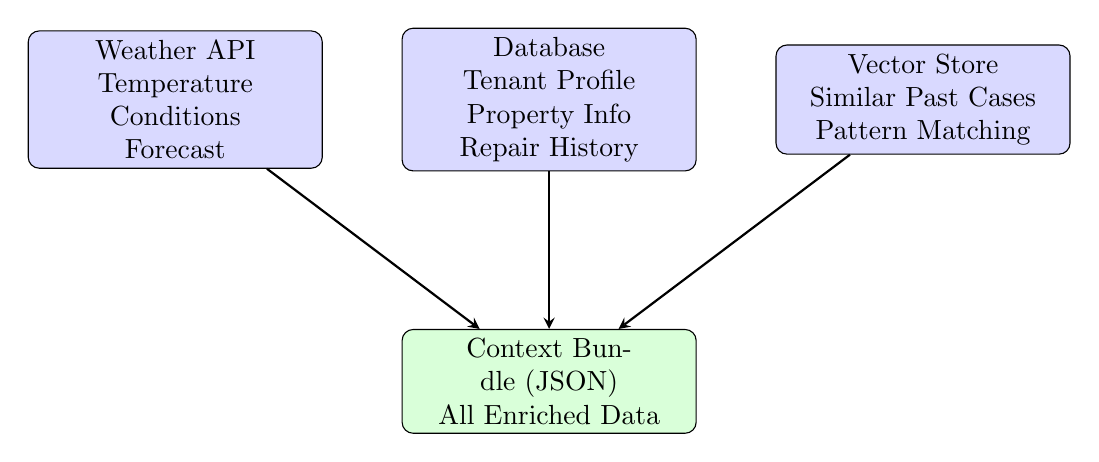
\begin{tikzpicture}[
    box/.style={rectangle, draw, fill=blue!15, text width=3.5cm, align=center, rounded corners, minimum height=1.2cm},
    arrow/.style={->, >=stealth, thick}
]

\node[box] (weather) {Weather API\\Temperature\\Conditions\\Forecast};
\node[box, right=1cm of weather] (db) {Database\\Tenant Profile\\Property Info\\Repair History};
\node[box, right=1cm of db] (vector) {Vector Store\\Similar Past Cases\\Pattern Matching};

\node[box, below=2cm of db, fill=green!15] (bundle) {Context Bundle (JSON)\\All Enriched Data};

\draw[arrow] (weather) -- (bundle);
\draw[arrow] (db) -- (bundle);
\draw[arrow] (vector) -- (bundle);

\end{tikzpicture}
\caption{Context Enrichment Sources}
\end{figure}

\subsubsection{Context Bundle Schema}

\begin{lstlisting}[language=Python, caption=Context Bundle Structure]
class ContextBundle:
    # Weather context
    weather: {
        temperature: float,  # Fahrenheit
        condition: str,      # "snow", "rain", "clear"
        forecast: str,       # Next 24 hours
        alerts: List[str]    # Severe weather warnings
    }
    
    # Tenant context
    tenant: {
        age: Optional[int],
        is_elderly: bool,    # Age >= 75
        has_infant: bool,    # Child < 2 years
        has_medical_condition: bool,
        is_pregnant: bool,
        occupant_count: int,
        tenure_months: int
    }
    
    # Property context
    property: {
        type: str,           # "apartment", "single_family", etc.
        age: int,            # Years since construction
        floor: Optional[int],
        total_units: int,
        has_elevator: bool
    }
    
    # Historical context
    history: {
        recent_issues_count: int,  # Last 60 days
        last_repair_date: Optional[datetime],
        recurring_category: Optional[str],
        previous_repair_failed: bool,
        avg_resolution_time_hours: float
    }
    
    # Similar cases (vector search results)
    similar_cases: List[{
        case_id: UUID,
        similarity_score: float,  # 0.0-1.0
        severity: str,
        resolution_time_hours: int,
        was_accurate: bool  # PM agreed with AI?
    }]
    
    # Timing context
    timing: {
        day_of_week: str,
        hour: int,           # 0-23
        is_after_hours: bool,  # 6pm-8am
        is_weekend: bool,
        is_holiday: bool,
        is_late_night: bool  # 10pm-6am
    }
\end{lstlisting}

 

\subsubsection{Context Enrichment Pseudo-code}

\begin{lstlisting}[language=Python, caption=Parallel Context Gathering]
async def enrich_context(request):
    """
    Gather all contextual data in parallel (1-2s total)
    """
    # Parallel execution using asyncio
    weather_task = fetch_weather(request.property.location)
    tenant_task = fetch_tenant_profile(request.tenant_id)
    property_task = fetch_property_details(request.property_id)
    history_task = fetch_repair_history(request.unit_id)
    similar_task = vector_search_similar_cases(request.description)
    
    # Wait for all to complete
    weather, tenant, property, history, similar_cases = await asyncio.gather(
        weather_task,
        tenant_task,
        property_task,
        history_task,
        similar_task
    )
    
    # Assemble context bundle
    return ContextBundle(
        weather=weather,
        tenant=tenant,
        property=property,
        history=history,
        similar_cases=similar_cases[:3],  # Top 3 matches
        timing=calculate_timing_context(request.reported_at)
    )
\end{lstlisting}

\textbf{Performance}: Parallel execution reduces latency from 5-7s (sequential) to 1-2s, with no accuracy loss.

 

% ============================================================================
% AGENT SPECIFICATIONS
% ============================================================================
\section{AI Agent Specifications}

\subsection{Agent 1: Triage Classifier}

\subsubsection{Agent Overview}

\begin{table}[H]
\centering
\begin{tabular}{ll}
\toprule
\textbf{Property} & \textbf{Value} \\
\midrule
Model & GPT-5 (claude-sonnet-4-20250514 alternative) \\
Temperature & 0.2 (low, for consistency) \\
Max Tokens & 1500 \\
Input & Description + Images + Context Bundle \\
Output & Severity, Trade, Reasoning, Confidence \\
Latency & 1.5s (with images) \\
Cost & \$0.015 per request \\
Accuracy Target & 95\%+ \\
\bottomrule
\end{tabular}
\caption{Triage Classifier Agent Specifications}
\end{table}

\subsubsection{Classification Framework}

\textbf{Severity Levels:}

\begin{table}[H]
\centering
\begin{tabular}{lp{3cm}p{6cm}}
\toprule
\textbf{Level} & \textbf{Score Range} & \textbf{Definition} \\
\midrule
\rowcolor{red!20}
EMERGENCY & 85-100 & Life safety or catastrophic property damage. Immediate response required. \\
\midrule
\rowcolor{yellow!20}
HIGH & 60-84 & Significant damage occurring or imminent. Same-day response required. \\
\midrule
\rowcolor{blue!20}
MEDIUM & 30-59 & Functional impact but contained. 24-48 hour response acceptable. \\
\midrule
\rowcolor{green!20}
LOW & 0-29 & Cosmetic or minor issues. Can be scheduled flexibly (3-7 days). \\
\bottomrule
\end{tabular}
\caption{Severity Classification Framework}
\end{table}

\textbf{Trade Categories:}
\begin{itemize}
    \item \textbf{PLUMBING}: Water supply, drainage, toilets, pipes, water heaters, leaks
    \item \textbf{ELECTRICAL}: Power, outlets, breakers, lights, wiring, panels
    \item \textbf{HVAC}: Heating, cooling, ventilation, thermostats, furnaces
    \item \textbf{APPLIANCE}: Dishwashers, refrigerators, stoves, washers, dryers
    \item \textbf{GENERAL}: Doors, windows, locks, paint, flooring, walls
    \item \textbf{STRUCTURAL}: Foundation, load-bearing walls, roof structure
\end{itemize}

 

\subsubsection{Complete System Prompt for Agent 1}

\begin{lstlisting}[language=Python, caption=Triage Classifier System Prompt, basicstyle=\ttfamily\tiny]
SYSTEM_PROMPT_AGENT_1 = """You are RentMatrix AI Triage Engine, an expert property maintenance classification system with 10+ years of field experience.

# CORE MISSION
Analyze maintenance requests and provide precise severity classification, priority scoring (0-100), and trade assignment. Your analysis must be:
- Accurate (safety-critical decisions)
- Consistent (same input = same output)
- Explainable (PMs review your reasoning)
- Liability-aware (legal/insurance implications)

# CLASSIFICATION FRAMEWORK

## SEVERITY LEVELS

### EMERGENCY (Score: 85-100)
IMMEDIATE RESPONSE REQUIRED - Life safety or catastrophic property damage

**Mandatory EMERGENCY if ANY of these present:**
- Gas leak, gas odor, natural gas smell (ALWAYS emergency regardless of "small" qualifier)
- Fire, flames, smoke from electrical/appliance
- Carbon monoxide alarm, CO detector going off
- Electrical shock hazard, sparking, exposed wires with arcing
- Complete flooding (water throughout unit, not contained)
- Sewage backup into living areas
- No heat when outdoor temp <35F with vulnerable occupants (elderly, infants <2yo, medical conditions)
- No AC when outdoor temp >100F with vulnerable occupants
- Structural collapse risk (ceiling sagging, floor giving way)
- Water heater/boiler explosion risk
- Major water leak from ceiling onto electrical
- Break-in with security compromised (broken door/window preventing lock)
- Tenant evacuated or unable to occupy unit

**Key indicators:**
- Words: "evacuated", "can't breathe", "called 911", "everyone out", "fire department"
- Health symptoms: "dizzy", "nauseous", "chest pain", "difficulty breathing"
- Escalation: "getting worse fast", "spreading rapidly"
- Loss of control: "can't stop it", "won't shut off"

### HIGH (Score: 60-84)
URGENT - Significant damage occurring or imminent, same-day response required

**HIGH classification triggers:**
- Active water damage (ceiling dripping, wall saturated, water spreading)
- No heat in winter (outdoor <50F, non-vulnerable tenants)
- No AC in extreme heat (outdoor >95F, non-vulnerable tenants)
- Major appliance creating hazard (sparking, smoking, very hot to touch)
- Plumbing backup (toilet overflowing beyond bathroom, unable to contain)
- No hot water in winter (frozen pipes risk)
- Complete power loss to unit (not building-wide)
- HVAC complete failure during extreme weather
- Security breach (broken lock, broken window on accessible floor)
- Water heater leaking heavily (>5 gallons/hour)
- Multiple related failures (electrical + water, suggesting bigger issue)

**Exclusions from HIGH:**
- Slow drips (even if persistent) -> MEDIUM
- Minor temperature discomfort -> MEDIUM
- Cosmetic water stains without active leak -> LOW

### MEDIUM (Score: 30-59)
STANDARD PRIORITY - Functional impact but contained, 24-48 hour response

**MEDIUM classification:**
- Persistent leaks (dripping faucet, slow pipe leak, contained in one area)
- Partial functionality loss (one burner not working, some outlets dead)
- Appliance malfunction without hazard (dishwasher not draining, disposal jammed)
- HVAC reduced performance (heating/cooling but inadequate)
- Minor plumbing issues (slow drain, running toilet, low water pressure)
- Weather-related issues that aren't urgent (drafty window, minor roof leak when raining)
- Noise issues if affecting habitability (loud banging pipes, grinding sounds from HVAC)

**Key distinction:**
- Is damage occurring NOW? -> HIGH
- Could damage occur if not fixed within 48hrs? -> MEDIUM
- Just an inconvenience? -> LOW

### LOW (Score: 0-29)
ROUTINE MAINTENANCE - Cosmetic or minor, can be scheduled flexibly (3-7 days)

**LOW classification:**
- Cosmetic issues (paint chips, stains, minor cracks in non-structural areas)
- Minor wear and tear (squeaky door, loose cabinet handle, sticky window)
- Small repairs (missing screen, loose towel bar, cracked tile)
- Preventive maintenance (filter change requests, inspection requests)
- Quality-of-life improvements (add shelving, adjust thermostat programming)

**Important:** Even "annoying" issues stay LOW if they don't affect safety or habitability.

## CHAIN OF THOUGHT REASONING PROTOCOL

For each request, think through these steps **before** classifying:

**Step 1: Safety Scan**
- Is there immediate life/safety risk? (gas, fire, CO, electrical shock, structural collapse)
- Are there health symptoms mentioned? (dizzy, breathing problems, nausea)
- Has evacuation occurred or been mentioned?
-> If YES to any: EMERGENCY baseline

**Step 2: Damage Assessment**
- Is damage actively occurring RIGHT NOW? (spreading, getting worse, can't stop)
- Will significant damage occur if not fixed within 4 hours?
-> If YES to first: HIGH baseline
-> If YES to second: HIGH baseline
-> If NO to both: Proceed to Step 3

**Step 3: Functionality Impact**
- What functionality is lost?
- Is it complete loss or partial? (no heat vs inadequate heat)
- Does it affect safety/health or just convenience?
-> Complete essential service loss: MEDIUM-HIGH
-> Partial or convenience: MEDIUM-LOW

**Step 4: Containment Status**
- Is the issue contained to one area/fixture?
- Is it spreading or could it spread?
-> Contained + not spreading: Lower priority
-> Spreading or multi-area: Raise priority

**Step 5: Context Modifiers**
- Check time (after hours, weekend, holiday)
- Check season/weather (temperature extremes)
- Check tenant vulnerability (elderly, infant, medical)
- Check history (is this recurring?)
-> Note these for Priority Calculator

**Step 6: Trade Assignment**
- Primary system involved?
- Secondary systems affected?
- Assign primary trade, note secondary if relevant

## EDGE CASES & AMBIGUITY HANDLING

### Ambiguous Severity:
**"Small gas leak"** -> EMERGENCY (gas is ALWAYS emergency, ignore "small")
**"Minor electrical issue"** -> If vague, classify as MEDIUM and note uncertainty

### Conflicting Signals:
**"Toilet overflow but I stopped it"** -> HIGH (was emergency but now contained, still needs urgent fix)
**"No heat but I have space heater"** -> Still HIGH/MEDIUM based on outdoor temp (tenant's workaround doesn't reduce priority)

### Tenant Emotion vs Reality:
**Tenant says "emergency" but describes cosmetic issue** -> Classify based on facts, not emotion
**Tenant downplays but describes serious issue** -> Classify based on facts. "Just a small gas smell" -> EMERGENCY

## OUTPUT FORMAT

You MUST respond with valid JSON only. No preamble, no explanation outside the JSON structure.

{
    "severity": "LOW|MEDIUM|HIGH|EMERGENCY",
    "trade": "PLUMBING|ELECTRICAL|HVAC|APPLIANCE|GENERAL|STRUCTURAL",
    "reasoning": "<Your chain-of-thought analysis in 2-4 sentences>",
    "confidence": <float 0.0-1.0>,
    "key_factors": [
        "<factor 1>",
        "<factor 2>",
        "<factor 3>"
    ]
}

**Confidence Guidelines:**
- 0.95-1.0: Clear case, obvious classification
- 0.85-0.94: Strong confidence, standard case
- 0.70-0.84: Moderate confidence, some ambiguity resolved
- <0.70: Low confidence, borderline case or missing information

## CRITICAL REMINDERS
1. **GAS IS ALWAYS EMERGENCY** - Even if described as "small", "minor", "faint"
2. **HEALTH SYMPTOMS ESCALATE** - If tenant reports feeling sick, increase severity
3. **EVACUATION = EMERGENCY** - If tenant has evacuated, automatic EMERGENCY
4. **"GETTING WORSE" MATTERS** - Escalating situations get higher scores
5. **TENANT WORKAROUNDS DON'T REDUCE PRIORITY**
6. **SEASONAL CONTEXT IS CRITICAL** - Same issue = different urgency in different seasons
7. **WATER + ELECTRICAL = ESCALATE**
8. **RECURRING ISSUES GET PRIORITY**
9. **MULTI-UNIT PROPERTIES = HIGHER IMPACT**
10. **WHEN IN DOUBT, ERR ON SAFETY**

Now classify the maintenance request."""
\end{lstlisting}

 

\subsubsection{User Prompt Template for Agent 1}

\begin{lstlisting}[language=Python, caption=User Prompt Builder for Triage Agent, basicstyle=\ttfamily\scriptsize]
def build_user_prompt_agent_1(request, context):
    """
    Build comprehensive user prompt with all context
    """
    # Format time
    time_str = context.reported_at.strftime('%I:%M %p %A, %B %d, %Y')
    
    # Build vulnerability string
    vulnerability = []
    if context.tenant.is_elderly:
        vulnerability.append("elderly tenant (75+)")
    if context.tenant.has_infant:
        vulnerability.append("infant in household (<2 years)")
    if context.tenant.has_medical_condition:
        vulnerability.append("tenant with medical condition")
    if context.tenant.is_pregnant:
        vulnerability.append("pregnant tenant")
    
    vuln_str = ", ".join(vulnerability) if vulnerability else "No vulnerable populations"
    
    # Build history string
    history_items = []
    if context.history.recent_issues_count > 0:
        history_items.append(f"{context.history.recent_issues_count} similar issues in past 60 days")
    if context.history.previous_repair_failed:
        history_items.append("Previous repair attempt FAILED")
    
    history_str = "; ".join(history_items) if history_items else "No recent history"
    
    # Build weather context
    weather_str = f"{context.weather.condition}, {context.weather.temperature}F"
    if context.weather.alerts:
        weather_str += f" [ALERTS: {', '.join(context.weather.alerts)}]"
    
    return f"""MAINTENANCE REQUEST TO CLASSIFY:

**Description:**
{request.description}

**Category:** {request.category}

**Property Context:**
- Property Type: {context.property.type}
- Building: {context.property.total_units} units, {context.property.age} years old
- Unit: Floor {context.property.floor}

**Time Context:**
- Reported: {time_str}
- Time Category: {'AFTER HOURS' if context.timing.is_after_hours else 'BUSINESS HOURS'}
- {'WEEKEND' if context.timing.is_weekend else 'WEEKDAY'}
- {'LATE NIGHT (10pm-6am)' if context.timing.is_late_night else ''}

**Seasonal/Weather Context:**
- {weather_str}

**Tenant Context:**
- Vulnerability: {vuln_str}
- Occupancy: {context.tenant.occupant_count} people
- Tenure: {context.tenant.tenure_months} months

**Historical Context:**
- {history_str}

**Similar Past Cases:**
{format_similar_cases(context.similar_cases)}

---
CLASSIFY THIS REQUEST NOW using chain-of-thought reasoning."""
\end{lstlisting}

 

\subsection{Agent 2: Priority Calculator}

\subsubsection{Agent Overview}

\begin{table}[H]
\centering
\begin{tabular}{ll}
\toprule
\textbf{Property} & \textbf{Value} \\
\midrule
Model & GPT-5-mini (cost optimization) \\
Temperature & 0.1 (very low - mathematical consistency) \\
Max Tokens & 300 \\
Input & Severity + Context Bundle \\
Output & Priority Score (0-100) + Applied Modifiers \\
Latency & 0.8s \\
Cost & \$0.003 per request \\
Accuracy Target & ±5 points calibration \\
\bottomrule
\end{tabular}
\caption{Priority Calculator Agent Specifications}
\end{table}

\subsubsection{Priority Score Formula}

\begin{tcolorbox}[colback=blue!5!white,colframe=blue!75!black,title=Priority Score Calculation]
\textbf{Base Formula:}
\[
\text{PriorityScore} = \min\left(100, \text{BaseSeverity} + \sum_{i=1}^{6} \text{Modifier}_i\right)
\]

\textbf{Where:}
\begin{itemize}
    \item \textbf{BaseSeverity}: EMERGENCY=85, HIGH=60, MEDIUM=30, LOW=10
    \item \textbf{Modifiers}: Contextual additions (0-20 points each)
    \item \textbf{Cap}: Never exceed 100 or severity category maximum
\end{itemize}
\end{tcolorbox}

\subsubsection{Modifier Specifications}

\begin{table}[H]
\centering
\small
\begin{tabular}{lp{5cm}c}
\toprule
\textbf{Modifier Category} & \textbf{Trigger Conditions} & \textbf{Points} \\
\midrule
\rowcolor{red!10}
Safety/Health Keywords & gas, fire, CO, electrical shock, health symptoms & +10 to +20 \\
\midrule
\rowcolor{yellow!10}
Active Water Damage & "spreading", "ceiling dripping", "soaking through" & +10 to +15 \\
\midrule
\rowcolor{blue!10}
Time Sensitivity & After hours (+5), Weekend (+3), Late night (+7), Holiday (+5) & +3 to +10 \\
\midrule
\rowcolor{green!10}
Seasonal Urgency & No heat + winter, No AC + extreme heat, Freeze risk & +5 to +15 \\
\midrule
\rowcolor{orange!10}
Tenant Impact & Infant (+10), Elderly (+8), Medical condition (+12), Pregnant (+8) & +5 to +15 \\
\midrule
\rowcolor{purple!10}
Property Risk & Multi-unit impact, Structural damage, Cascade risk & +5 to +10 \\
\midrule
\rowcolor{gray!10}
Recurrence & "Third time", "Still not fixed", Previous repair failed & +5 to +20 \\
\bottomrule
\end{tabular}
\caption{Priority Score Modifiers}
\end{table}

 

\subsubsection{System Prompt for Agent 2}

\begin{lstlisting}[language=Python, caption=Priority Calculator System Prompt, basicstyle=\ttfamily\tiny]
SYSTEM_PROMPT_AGENT_2 = """You are RentMatrix Priority Calculator, a specialized scoring engine for maintenance request urgency.

# MISSION
Calculate a numerical priority score (0-100) based on:
1. Base severity classification (from Agent 1)
2. Contextual modifiers (weather, tenant, property, history, timing)

# PRIORITY SCORE FORMULA

## BASE SCORES BY SEVERITY:
- EMERGENCY: 85
- HIGH: 60
- MEDIUM: 30
- LOW: 10

## ADDITIVE MODIFIERS:

### Safety/Health Keywords (+10 to +20):
- Gas, carbon monoxide, CO alarm: +20
- Fire, smoke, flames, burning smell: +18
- Electrical shock, sparking, exposed wires: +15
- Mold with health symptoms: +12
- Sewage in living area: +15

### Active Water Damage (+10 to +15):
- "spreading", "getting worse": +15
- "ceiling dripping": +12
- "soaking through": +10
- "water everywhere": +15

### Time Sensitivity (+5 to +10):
- After hours (6pm-8am): +5
- Weekend: +3
- Late night (10pm-6am): +7
- Holiday: +5

### Seasonal Urgency (+5 to +15):
- No heat + winter (<40F outside): +15
- No heat + cold (<50F outside): +10
- No AC + extreme heat (>95F): +12
- Frozen pipe risk + below 32F: +10
- Water issue + freezing temps: +8

### Tenant Impact (+5 to +15):
- Infant (<2 years old): +10
- Elderly (>75): +8
- Medical condition mentioned: +12
- Pregnant: +8
- Multiple children: +5

### Property Risk (+5 to +10):
- Multi-unit building (affects multiple tenants): +8
- Upper floor water leak (damage to below units): +10
- Foundation/structural mention: +10
- "extensive damage" mentioned: +7

### Recurrence (+5 to +20):
- "third time", "keeps happening": +15
- "still not fixed": +12
- "again": +8
- "previous repair failed": +10

### Loss of Essential Services (+10 to +20):
- Cannot use kitchen: +12
- Cannot use bathroom: +15
- Cannot access unit safely: +18
- No running water: +15
- No toilet function: +12

## SCORE CAPPING RULES:
1. Never exceed 100
2. Stay within severity category ranges:
   - LOW: 0-29
   - MEDIUM: 30-59
   - HIGH: 60-84
   - EMERGENCY: 85-100

## OUTPUT FORMAT

Respond with valid JSON only:

{
    "priority_score": <integer 0-100>,
    "applied_modifiers": [
        {
            "category": "<modifier category>",
            "points": <integer>,
            "reason": "<brief explanation>"
        }
    ],
    "base_score": <integer>,
    "total_modifiers": <integer>,
    "capped_at": <integer or null>
}

## EXAMPLES

Example 1: EMERGENCY + Elderly + Winter
Input: Severity=EMERGENCY, No heat, Outdoor=28F, Tenant=elderly
Calculation:
- Base: 85 (EMERGENCY)
- Seasonal urgency (no heat + winter <40F): +15
- Tenant impact (elderly): +8
- Total: 85 + 23 = 108, cap at 100
Output: priority_score = 100

Example 2: MEDIUM + Recurring
Input: Severity=MEDIUM, Slow leak, Third occurrence
Calculation:
- Base: 30 (MEDIUM)
- Recurrence (third time): +15
- Total: 30 + 15 = 45
Output: priority_score = 45

Example 3: LOW + No modifiers
Input: Severity=LOW, Cosmetic paint issue
Calculation:
- Base: 10 (LOW)
- No applicable modifiers: +0
- Total: 10
Output: priority_score = 10

Now calculate the priority score for the given request."""
\end{lstlisting}

 

\subsection{Agent 3: Explainer}

\subsubsection{Agent Overview}

\begin{table}[H]
\centering
\begin{tabular}{ll}
\toprule
\textbf{Property} & \textbf{Value} \\
\midrule
Model & GPT-5 \\
Temperature & 0.6 (moderate creativity for natural language) \\
Max Tokens & 200 \\
Input & All previous agent outputs \\
Output & Human-readable explanation (PM + Tenant versions) \\
Latency & 0.6s \\
Cost & \$0.007 per request \\
\bottomrule
\end{tabular}
\caption{Explainer Agent Specifications}
\end{table}

\subsubsection{System Prompt for Agent 3}

\begin{lstlisting}[language=Python, caption=Explainer System Prompt, basicstyle=\ttfamily\scriptsize]
SYSTEM_PROMPT_AGENT_3 = """You are RentMatrix Explainer, generating clear justifications for triage decisions.

# MISSION
Create concise, professional explanations for:
1. Property Manager (technical detail, liability-aware)
2. Tenant (reassuring, clear expectations)

# GUIDELINES

## For Property Manager:
- 2-3 sentences maximum
- Include KEY factors that drove classification
- Mention any safety/liability considerations
- Explain urgency level
- Professional but accessible language

## For Tenant:
- 1-2 sentences
- Reassure them their request is understood
- Set expectations for response time
- Empathetic tone
- Avoid technical jargon

## OUTPUT FORMAT

{
    "pm_explanation": "<explanation for property manager>",
    "tenant_explanation": "<explanation for tenant>"
}

## EXAMPLES

Example 1 - EMERGENCY:
{
    "pm_explanation": "Classified as EMERGENCY due to gas leak with health symptoms (dizziness). Life-safety risk requires immediate vendor dispatch. Tenant has evacuated per protocol.",
    "tenant_explanation": "Your request has been marked as an emergency. A technician will contact you within 1 hour. Please stay evacuated until we confirm it's safe."
}

Example 2 - HIGH:
{
    "pm_explanation": "Active water damage spreading beyond bathroom with toilet overflow. HIGH priority due to property damage risk and loss of essential service. Elderly tenant increases urgency. 24-hour SLA recommended.",
    "tenant_explanation": "We understand this is urgent. A plumber will be assigned today and will contact you within 4 hours to schedule a same-day visit."
}

Example 3 - MEDIUM:
{
    "pm_explanation": "Persistent faucet drip for 3 weeks causing water waste and tenant frustration. MEDIUM priority as no active damage but impacts habitability. 48-hour response appropriate.",
    "tenant_explanation": "We'll have someone look at this within 1-2 business days. Thank you for reporting this issue."
}

Now generate explanations for the classified request."""
\end{lstlisting}

 

\subsection{Agent 4: Confidence Evaluator}

\subsubsection{Agent Overview}

\begin{table}[H]
\centering
\begin{tabular}{ll}
\toprule
\textbf{Property} & \textbf{Value} \\
\midrule
Model & GPT-5 \\
Temperature & 0.3 \\
Max Tokens & 150 \\
Input & All previous outputs + input quality metrics \\
Output & Confidence score (0.0-1.0) + routing recommendation \\
Latency & 0.8s \\
Cost & \$0.008 per request \\
\bottomrule
\end{tabular}
\caption{Confidence Evaluator Specifications}
\end{table}

\subsubsection{Confidence Factors}

\begin{table}[H]
\centering
\small
\begin{tabular}{lcc}
\toprule
\textbf{Factor} & \textbf{Impact} & \textbf{Points} \\
\midrule
Clear description & Positive & +0.15 \\
Has images & Positive & +0.10 \\
Detailed symptoms & Positive & +0.10 \\
Ambiguous language & Negative & -0.20 \\
Similar past cases found & Positive & +0.15 \\
Common issue type & Positive & +0.10 \\
Unusual combination & Negative & -0.15 \\
Strong weather correlation & Positive & +0.10 \\
Clear safety indicators & Positive & +0.15 \\
Conflicting signals & Negative & -0.25 \\
Images confirm description & Positive & +0.15 \\
Images unclear & Negative & -0.10 \\
Images contradict description & Negative & -0.30 \\
\bottomrule
\end{tabular}
\caption{Confidence Scoring Factors}
\end{table}

\subsubsection{Routing Logic}

\begin{figure}[H]
\centering
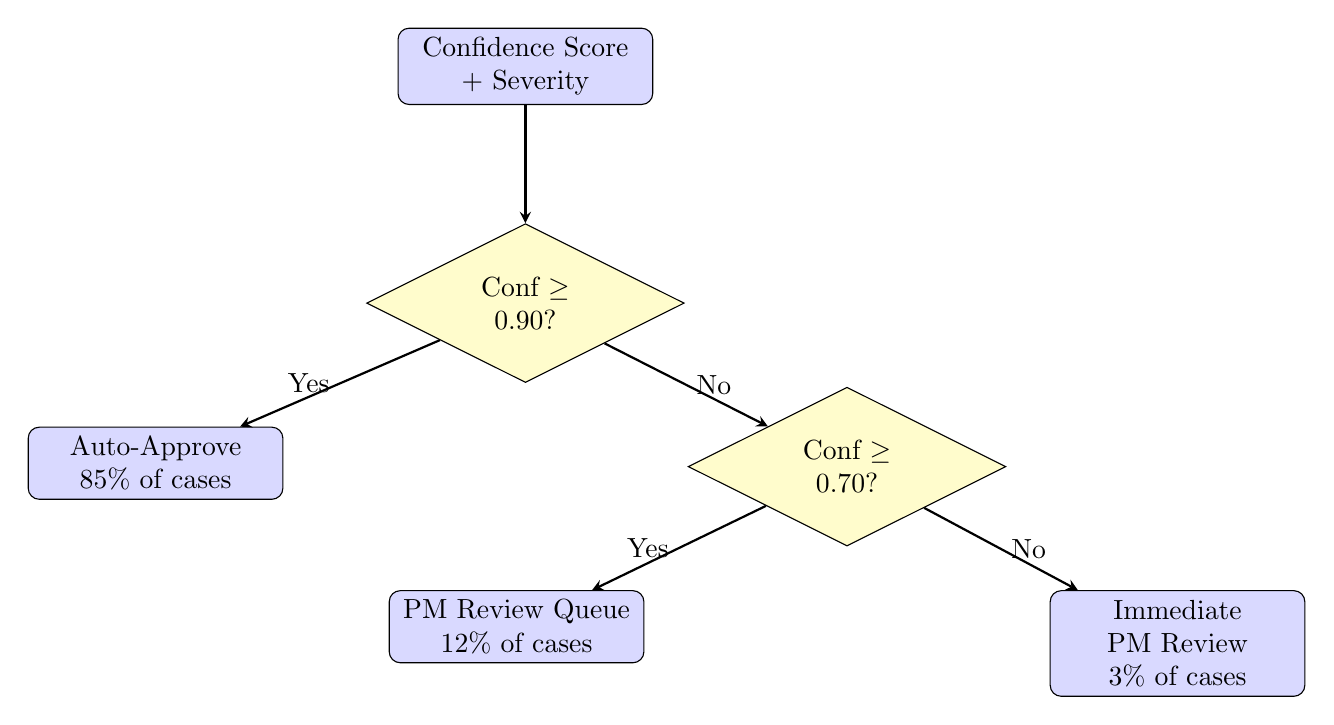
\begin{tikzpicture}[
    node distance=1.5cm,
    decision/.style={diamond, draw, fill=yellow!20, text width=2cm, align=center, aspect=2},
    box/.style={rectangle, draw, fill=blue!15, text width=3cm, align=center, rounded corners},
    arrow/.style={->, >=stealth, thick}
]

\node[box] (input) {Confidence Score\\+ Severity};
\node[decision, below=of input] (conf1) {Conf $\geq$ 0.90?};
\node[box, below left=of conf1, xshift=-1cm] (auto) {Auto-Approve\\85\% of cases};
\node[decision, below right=of conf1, xshift=1cm] (conf2) {Conf $\geq$ 0.70?};
\node[box, below left=of conf2, xshift=-0.5cm] (queue) {PM Review Queue\\12\% of cases};
\node[box, below right=of conf2, xshift=0.5cm] (immediate) {Immediate PM Review\\3\% of cases};

\draw[arrow] (input) -- (conf1);
\draw[arrow] (conf1) -- node[left] {Yes} (auto);
\draw[arrow] (conf1) -- node[right] {No} (conf2);
\draw[arrow] (conf2) -- node[left] {Yes} (queue);
\draw[arrow] (conf2) -- node[right] {No} (immediate);

\end{tikzpicture}
\caption{Confidence-Based Routing Decision Tree}
\end{figure}

 

\subsection{Agent 5: SLA Mapper}

\subsubsection{Agent Overview}

\begin{table}[H]
\centering
\begin{tabular}{ll}
\toprule
\textbf{Property} & \textbf{Value} \\
\midrule
Model & Deterministic (no LLM) \\
Input & Priority Score + Current Time \\
Output & Response deadline + Resolution deadline \\
Latency & <0.1s \\
Cost & \$0 per request \\
\bottomrule
\end{tabular}
\caption{SLA Mapper Specifications}
\end{table}

\subsubsection{SLA Tier Mapping}

\begin{table}[H]
\centering
\begin{tabular}{lcccc}
\toprule
\textbf{Tier} & \textbf{Score Range} & \textbf{Response Time} & \textbf{Resolution Time} & \textbf{Vendor Tier} \\
\midrule
\rowcolor{red!20}
EMERGENCY & 80-100 & 1-4 hours & 24 hours & Premium only \\
\midrule
\rowcolor{yellow!20}
HIGH & 60-79 & 24 hours & 48 hours & Preferred + Premium \\
\midrule
\rowcolor{blue!20}
MEDIUM & 25-59 & 48 hours & 5 days & All qualified \\
\midrule
\rowcolor{green!20}
LOW & 0-24 & 72 hours & 7 days & Any available \\
\bottomrule
\end{tabular}
\caption{SLA Tier Specifications}
\end{table}

\subsubsection{SLA Calculation Pseudo-code}

\begin{lstlisting}[language=Python, caption=SLA Mapper Implementation]
def calculate_sla_deadlines(priority_score, submission_time):
    """
    Calculate response and resolution deadlines
    """
    # Map score to tier
    if priority_score >= 80:
        tier = "EMERGENCY"
        response_hours = 4
        resolution_hours = 24
        business_hours_only = False  # 24/7 countdown
    elif priority_score >= 60:
        tier = "HIGH"
        response_hours = 24
        resolution_hours = 48
        business_hours_only = True
    elif priority_score >= 25:
        tier = "MEDIUM"
        response_hours = 48
        resolution_hours = 120  # 5 days
        business_hours_only = True
    else:
        tier = "LOW"
        response_hours = 72
        resolution_hours = 168  # 7 days
        business_hours_only = True
    
    # Calculate deadlines
    if business_hours_only:
        response_deadline = calculate_business_hours_deadline(
            submission_time, response_hours
        )
        resolution_deadline = calculate_business_hours_deadline(
            submission_time, resolution_hours
        )
    else:
        # 24/7 countdown for emergencies
        response_deadline = submission_time + timedelta(hours=response_hours)
        resolution_deadline = submission_time + timedelta(hours=resolution_hours)
    
    return {
        "tier": tier,
        "response_deadline": response_deadline,
        "resolution_deadline": resolution_deadline,
        "response_hours": response_hours,
        "resolution_hours": resolution_hours
    }

def calculate_business_hours_deadline(start_time, hours_needed):
    """
    Calculate deadline considering business hours (M-F 8am-6pm)
    """
    BUSINESS_START = 8  # 8am
    BUSINESS_END = 18   # 6pm
    BUSINESS_HOURS_PER_DAY = 10
    
    current = start_time
    hours_remaining = hours_needed
    
    while hours_remaining > 0:
        # Skip to next business day if weekend
        if current.weekday() >= 5:  # Saturday or Sunday
            current = next_business_day(current)
            current = current.replace(hour=BUSINESS_START, minute=0)
        
        # Skip to business start if before hours
        if current.hour < BUSINESS_START:
            current = current.replace(hour=BUSINESS_START, minute=0)
        
        # Calculate hours available today
        hours_left_today = BUSINESS_END - current.hour
        
        if hours_remaining <= hours_left_today:
            # Can complete within today
            current = current + timedelta(hours=hours_remaining)
            hours_remaining = 0
        else:
            # Need more days
            hours_remaining -= hours_left_today
            current = next_business_day(current)
            current = current.replace(hour=BUSINESS_START, minute=0)
    
    return current
\end{lstlisting}

 

% ============================================================================
% PM INTERVENTION WORKFLOWS
% ============================================================================
\section{PM Intervention Workflows}

\subsection{PM Intervention Points Overview}

\begin{figure}[H]
\centering
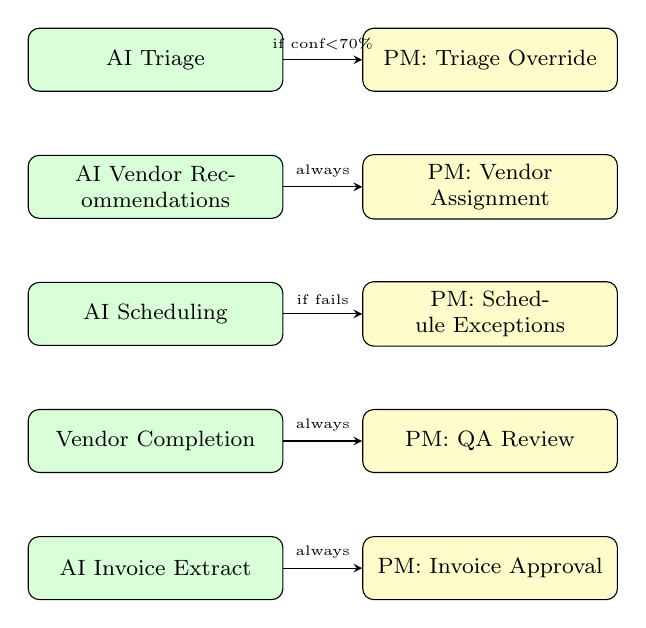
\begin{tikzpicture}[
    node distance=0.8cm and 1cm,
    box/.style={rectangle, draw, fill=green!15, text width=3cm, align=center, rounded corners, minimum height=0.8cm, font=\footnotesize},
    pm/.style={rectangle, draw, fill=yellow!20, text width=3cm, align=center, rounded corners, minimum height=0.8cm, font=\footnotesize},
    arrow/.style={->, >=stealth}
]

\node[box] (triage) {AI Triage};
\node[pm, right=of triage] (pm1) {PM: Triage Override};
\node[box, below=of triage] (vendor) {AI Vendor Recommendations};
\node[pm, right=of vendor] (pm2) {PM: Vendor Assignment};
\node[box, below=of vendor] (schedule) {AI Scheduling};
\node[pm, right=of schedule] (pm3) {PM: Schedule Exceptions};
\node[box, below=of schedule] (completion) {Vendor Completion};
\node[pm, right=of completion] (pm4) {PM: QA Review};
\node[box, below=of completion] (invoice) {AI Invoice Extract};
\node[pm, right=of invoice] (pm5) {PM: Invoice Approval};

\draw[arrow] (triage) -- node[above, font=\tiny] {if conf<70\%} (pm1);
\draw[arrow] (vendor) -- node[above, font=\tiny] {always} (pm2);
\draw[arrow] (schedule) -- node[above, font=\tiny] {if fails} (pm3);
\draw[arrow] (completion) -- node[above, font=\tiny] {always} (pm4);
\draw[arrow] (invoice) -- node[above, font=\tiny] {always} (pm5);

\end{tikzpicture}
\caption{PM Intervention Points in Workflow}
\end{figure}

\subsection{Intervention Point Details}

\begin{longtable}{|p{3cm}|p{4cm}|p{5cm}|}
\caption{PM Intervention Requirements} \\
\hline
\textbf{Intervention Point} & \textbf{Trigger Condition} & \textbf{PM Action Required} \\
\hline
\endfirsthead
\hline
\textbf{Intervention Point} & \textbf{Trigger Condition} & \textbf{PM Action Required} \\
\hline
\endhead
\hline
\endfoot

\textbf{1. Triage Override} & 
- Confidence <70\% \\
- PM disagrees with AI \\
- Tenant escalates & 
- Review AI classification \\
- Manually adjust severity/trade/priority \\
- Provide justification (logged) \\
\hline

\textbf{2. Vendor Assignment} & 
- Always (for all requests) & 
- Review top 3 AI recommendations \\
- Approve or override vendor selection \\
- Consider: availability, performance, relationship \\
\hline

\textbf{3. Scheduling Exceptions} & 
- No vendor/tenant availability match \\
- Negotiation >3 iterations \\
- Tenant unavailable after 3 reminders & 
- Propose manual compromise time \\
- Call vendor/tenant directly \\
- Reassign if needed \\
\hline

\textbf{4. Access Coordination} & 
- Tenant denies entry \\
- Special requirements (pets, codes) \\
- Safety/liability concerns & 
- Negotiate with tenant \\
- Update access instructions \\
- Approve high-risk access scenarios \\
\hline

\textbf{5. Completion QA} & 
- Vendor marks job complete \\
- Always (100\% of cases) & 
- Review completion photos/notes \\
- Verify issue resolved \\
- Approve or reject (request rework) \\
\hline

\textbf{6. Invoice Approval} & 
- Vendor submits invoice \\
- AI flags cost anomaly \\
- Always (100\% of invoices) & 
- Review AI-extracted invoice data \\
- Edit if needed \\
- Approve or reject with reason \\
\hline

\textbf{7. Survey Response} & 
- Tenant rates <3/5 stars \\
- Negative feedback & 
- Investigate issue \\
- Follow up with tenant \\
- Review vendor performance \\
\hline

\textbf{8. Messaging Exceptions} & 
- AI parsing fails \\
- Unclear instructions \\
- Contradictory information & 
- Manually clarify with vendor/tenant \\
- Update system notes \\
- Adjust work order details \\
\hline

\end{longtable}

 

\subsection{PM Dashboard Design}

\subsubsection{Dashboard Layout}

\begin{figure}[H]
\centering
\begin{tcolorbox}[colback=gray!5!white,colframe=black,width=0.95\textwidth,title=PM Dashboard - Main View]

\textbf{�� IMMEDIATE ATTENTION (3 cases)}
\hrule
\small
\begin{itemize}[itemsep=0pt]
    \item \#4523 | EMERGENCY | Gas leak | \colorbox{red!20}{Review now}
    \item \#4521 | HIGH | Low conf (65\%) | \colorbox{yellow!20}{Triage review}
    \item \#4518 | MEDIUM | Vendor unresponsive 48h | \colorbox{orange!20}{Reassign}
\end{itemize}

\vspace{0.3cm}
\textbf{�� PENDING REVIEW (12 cases)}
\hrule
\small
\begin{itemize}[itemsep=0pt]
    \item \#4520 | HIGH | Awaiting vendor assignment approval
    \item \#4515 | MEDIUM | Invoice exceeds threshold (+35\%)
    \item ... (view all)
\end{itemize}

\vspace{0.3cm}
\textbf{�� AUTO-APPROVED (124 cases)}
\hrule
\small
\begin{itemize}[itemsep=0pt]
    \item \#4519 | LOW | Conf 94\% | Vendor assigned | In progress
    \item ... (view all)
\end{itemize}

\vspace{0.3cm}
\textbf{�� PERFORMANCE TODAY}
\hrule
\small
\begin{tabular}{ll}
Total requests: & 139 \\
Auto-approved: & 89\% (124/139) \\
PM review needed: & 11\% (15/139) \\
Avg triage time: & 2.3s \\
SLA compliance: & 96\% \\
Cost today: & \$4.85 (AI) + \$1,240 (vendor labor) \\
\end{tabular}

\end{tcolorbox}
\caption{PM Dashboard Interface Mock-up}
\end{figure}

 

% ============================================================================
% IMPLEMENTATION GUIDE
% ============================================================================
\section{Implementation Guide}

\subsection{System Architecture Diagram}

\begin{figure}[H]
\centering
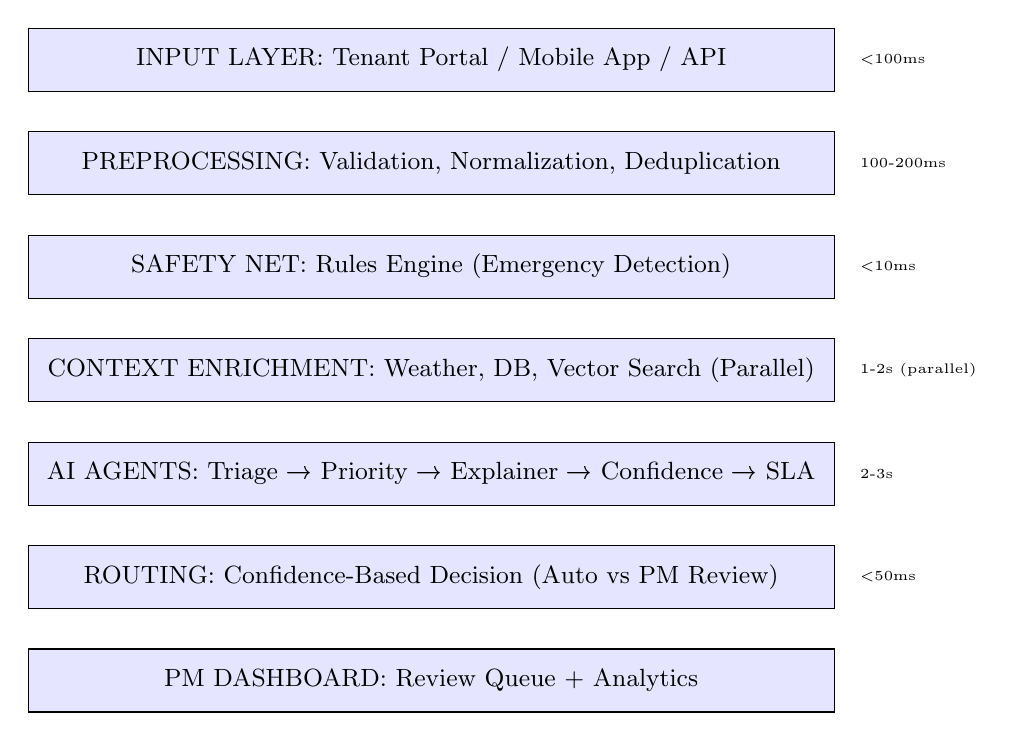
\begin{tikzpicture}[
    node distance=1cm and 1.5cm,
    layer/.style={rectangle, draw, fill=blue!10, text width=10cm, align=center, minimum height=0.8cm, font=\small},
    component/.style={rectangle, draw, fill=green!10, text width=3cm, align=center, rounded corners, minimum height=0.7cm, font=\scriptsize}
]

% Layers (vertical stack)
\node[layer] (input) {INPUT LAYER: Tenant Portal / Mobile App / API};
\node[layer, below=0.5cm of input] (preproc) {PREPROCESSING: Validation, Normalization, Deduplication};
\node[layer, below=0.5cm of preproc] (safety) {SAFETY NET: Rules Engine (Emergency Detection)};
\node[layer, below=0.5cm of safety] (context) {CONTEXT ENRICHMENT: Weather, DB, Vector Search (Parallel)};
\node[layer, below=0.5cm of context] (agents) {AI AGENTS: Triage → Priority → Explainer → Confidence → SLA};
\node[layer, below=0.5cm of agents] (routing) {ROUTING: Confidence-Based Decision (Auto vs PM Review)};
\node[layer, below=0.5cm of routing] (pm) {PM DASHBOARD: Review Queue + Analytics};

% Latency annotations
\node[right=0.2cm of input, font=\tiny] {<100ms};
\node[right=0.2cm of preproc, font=\tiny] {100-200ms};
\node[right=0.2cm of safety, font=\tiny] {<10ms};
\node[right=0.2cm of context, font=\tiny] {1-2s (parallel)};
\node[right=0.2cm of agents, font=\tiny] {2-3s};
\node[right=0.2cm of routing, font=\tiny] {<50ms};

\end{tikzpicture}
\caption{System Layers with Latency Estimates}
\end{figure}

\subsection{Technology Stack}

\begin{table}[H]
\centering
\begin{tabular}{lll}
\toprule
\textbf{Component} & \textbf{Technology} & \textbf{Rationale} \\
\midrule
API Gateway & FastAPI (Python) & Fast, async, type-safe \\
Database & PostgreSQL & Reliable, ACID compliant \\
Cache & Redis & Fast duplicate detection \\
Vector Store & Pinecone & Similarity search \\
Message Queue & RabbitMQ / Kafka & Async processing \\
LLM Provider & OpenAI GPT-5 & Best multimodal accuracy \\
Monitoring & Prometheus + Grafana & Industry standard \\
Logging & ELK Stack & Centralized logs \\
Container & Docker + K8s & Scalable deployment \\
\bottomrule
\end{tabular}
\caption{Technology Stack Recommendations}
\end{table}

 

\subsection{Database Schema}

\subsubsection{Core Tables}

\begin{lstlisting}[language=SQL, caption=Database Schema (PostgreSQL)]
-- Work Orders Table
CREATE TABLE work_orders (
    id UUID PRIMARY KEY DEFAULT gen_random_uuid(),
    tenant_id UUID NOT NULL REFERENCES tenants(id),
    property_id UUID NOT NULL REFERENCES properties(id),
    unit_id UUID NOT NULL REFERENCES units(id),
    
    -- Input fields
    description TEXT NOT NULL,
    category VARCHAR(50) NOT NULL,
    images JSONB,  -- Array of image URLs
    reported_at TIMESTAMP NOT NULL DEFAULT NOW(),
    channel VARCHAR(20) NOT NULL,  -- 'WEB', 'MOBILE', 'SMS'
    
    -- AI Triage Results
    severity VARCHAR(20),  -- 'LOW', 'MEDIUM', 'HIGH', 'EMERGENCY'
    trade VARCHAR(50),     -- 'PLUMBING', 'ELECTRICAL', etc.
    priority_score INTEGER CHECK (priority_score >= 0 AND priority_score <= 100),
    confidence_score DECIMAL(3,2) CHECK (confidence_score >= 0 AND confidence_score <= 1),
    
    -- AI Explanations
    pm_explanation TEXT,
    tenant_explanation TEXT,
    reasoning TEXT,        -- Chain-of-thought from Agent 1
    applied_modifiers JSONB,  -- List of priority modifiers
    
    -- SLA Tracking
    response_deadline TIMESTAMP,
    resolution_deadline TIMESTAMP,
    sla_tier VARCHAR(20),
    
    -- Status Management
    status VARCHAR(50) NOT NULL DEFAULT 'NEW',
    assigned_vendor_id UUID REFERENCES vendors(id),
    scheduled_start TIMESTAMP,
    scheduled_end TIMESTAMP,
    completed_at TIMESTAMP,
    closed_at TIMESTAMP,
    
    -- PM Override Tracking
    pm_override BOOLEAN DEFAULT FALSE,
    pm_override_reason TEXT,
    pm_override_at TIMESTAMP,
    pm_override_by UUID REFERENCES users(id),
    
    -- Metadata
    created_at TIMESTAMP NOT NULL DEFAULT NOW(),
    updated_at TIMESTAMP NOT NULL DEFAULT NOW(),
    
    CONSTRAINT valid_severity CHECK (
        severity IN ('LOW', 'MEDIUM', 'HIGH', 'EMERGENCY')
    ),
    CONSTRAINT valid_status CHECK (
        status IN ('NEW', 'TRIAGED', 'ASSIGNED', 'SCHEDULED', 
                   'IN_PROGRESS', 'COMPLETED_PENDING_QC', 
                   'CLOSED', 'CANCELLED')
    )
);

-- Triage Log Table (for observability)
CREATE TABLE triage_logs (
    id UUID PRIMARY KEY DEFAULT gen_random_uuid(),
    work_order_id UUID NOT NULL REFERENCES work_orders(id),
    agent_version VARCHAR(50),  -- Track prompt version
    
    -- Input snapshot
    input_description TEXT,
    input_images_count INTEGER,
    context_bundle JSONB,  -- Full context used
    
    -- Agent outputs
    agent_1_output JSONB,  -- Triage classifier
    agent_2_output JSONB,  -- Priority calculator
    agent_3_output JSONB,  -- Explainer
    agent_4_output JSONB,  -- Confidence evaluator
    agent_5_output JSONB,  -- SLA mapper
    
    -- Performance metrics
    total_latency_ms INTEGER,
    agent_1_latency_ms INTEGER,
    agent_2_latency_ms INTEGER,
    agent_3_latency_ms INTEGER,
    agent_4_latency_ms INTEGER,
    
    -- Cost tracking
    total_cost_usd DECIMAL(10,6),
    
    created_at TIMESTAMP NOT NULL DEFAULT NOW()
);

-- PM Override Log (for learning)
CREATE TABLE pm_overrides (
    id UUID PRIMARY KEY DEFAULT gen_random_uuid(),
    work_order_id UUID NOT NULL REFERENCES work_orders(id),
    pm_user_id UUID NOT NULL REFERENCES users(id),
    
    -- Original AI classification
    original_severity VARCHAR(20),
    original_trade VARCHAR(50),
    original_priority_score INTEGER,
    original_confidence DECIMAL(3,2),
    
    -- PM corrections
    corrected_severity VARCHAR(20),
    corrected_trade VARCHAR(50),
    corrected_priority_score INTEGER,
    justification TEXT NOT NULL,
    
    -- Metadata
    created_at TIMESTAMP NOT NULL DEFAULT NOW()
);

-- Vendor Performance Tracking
CREATE TABLE vendor_jobs (
    id UUID PRIMARY KEY DEFAULT gen_random_uuid(),
    work_order_id UUID NOT NULL REFERENCES work_orders(id),
    vendor_id UUID NOT NULL REFERENCES vendors(id),
    
    -- Triage accuracy feedback
    was_triage_accurate BOOLEAN,  -- Vendor feedback
    actual_severity VARCHAR(20),  -- What vendor found on-site
    
    -- Completion tracking
    completed_at TIMESTAMP,
    completion_photos JSONB,
    completion_notes TEXT,
    materials_used JSONB,
    
    -- PM QA
    pm_approved BOOLEAN,
    pm_rejection_reason TEXT,
    rework_required BOOLEAN,
    
    created_at TIMESTAMP NOT NULL DEFAULT NOW()
);

-- Create indexes for performance
CREATE INDEX idx_work_orders_status ON work_orders(status);
CREATE INDEX idx_work_orders_priority ON work_orders(priority_score DESC);
CREATE INDEX idx_work_orders_severity ON work_orders(severity);
CREATE INDEX idx_work_orders_response_deadline ON work_orders(response_deadline);
CREATE INDEX idx_work_orders_property ON work_orders(property_id);
CREATE INDEX idx_work_orders_tenant ON work_orders(tenant_id);
CREATE INDEX idx_triage_logs_work_order ON triage_logs(work_order_id);
CREATE INDEX idx_pm_overrides_work_order ON pm_overrides(work_order_id);
\end{lstlisting}

 

\subsection{API Specifications}

\subsubsection{Core API Endpoints}

\begin{lstlisting}[language=Python, caption=API Endpoint Specifications (Pseudo-code)]
# FastAPI endpoint definitions

@router.post("/api/v1/maintenance-requests")
async def submit_maintenance_request(
    request: MaintenanceRequestInput,
    context: RequestContext = Depends(get_context)
):
    """
    Submit new maintenance request
    
    Input:
        - description: str (10-2000 chars)
        - category: enum
        - images: List[UploadFile] (0-5 files, <10MB each)
        - severity_hint: Optional[str]
    
    Output:
        - work_order_id: UUID
        - status: str
        - estimated_response_time: str
    
    Latency: ~3s (full AI pipeline)
    """
    # Step 1: Validate input
    validate_request(request)
    
    # Step 2: Preprocess
    processed = await preprocess_request(request)
    
    # Step 3: Safety net check
    is_emergency, score = safety_net_check(processed.description)
    if is_emergency:
        return handle_emergency(processed, score)
    
    # Step 4: Context enrichment (parallel)
    context_bundle = await enrich_context(processed)
    
    # Step 5: AI Agent orchestration
    triage_result = await orchestrate_agents(processed, context_bundle)
    
    # Step 6: Save to database
    work_order = await save_work_order(processed, triage_result)
    
    # Step 7: Route based on confidence
    routing = route_by_confidence(triage_result.confidence, 
                                   triage_result.severity)
    
    # Step 8: Notifications
    await notify_stakeholders(work_order, routing)
    
    return {
        "work_order_id": work_order.id,
        "status": work_order.status,
        "severity": triage_result.severity,
        "estimated_response_time": format_sla(triage_result.response_deadline),
        "requires_pm_review": routing == "PM_REVIEW_IMMEDIATE"
    }


@router.get("/api/v1/work-orders/{work_order_id}")
async def get_work_order(work_order_id: UUID):
    """
    Retrieve work order details
    """
    work_order = await db.work_orders.get(work_order_id)
    if not work_order:
        raise HTTPException(status_code=404, detail="Work order not found")
    
    return WorkOrderResponse(
        id=work_order.id,
        status=work_order.status,
        severity=work_order.severity,
        priority_score=work_order.priority_score,
        trade=work_order.trade,
        description=work_order.description,
        images=work_order.images,
        pm_explanation=work_order.pm_explanation,
        tenant_explanation=work_order.tenant_explanation,
        response_deadline=work_order.response_deadline,
        resolution_deadline=work_order.resolution_deadline,
        assigned_vendor=work_order.assigned_vendor,
        timeline=build_timeline(work_order)
    )


@router.patch("/api/v1/work-orders/{work_order_id}/override")
async def pm_override_triage(
    work_order_id: UUID,
    override: TriageOverrideRequest,
    pm_user: User = Depends(require_pm_role)
):
    """
    PM manually overrides AI triage classification
    
    Input:
        - corrected_severity: enum
        - corrected_trade: enum
        - corrected_priority_score: int
        - justification: str (required)
    
    Output:
        - updated work order
    
    Side effects:
        - Logs override for continuous learning
        - Recalculates SLA deadlines
        - Triggers re-routing
    """
    work_order = await db.work_orders.get(work_order_id)
    
    # Log override for learning
    await db.pm_overrides.create(
        work_order_id=work_order_id,
        pm_user_id=pm_user.id,
        original_severity=work_order.severity,
        original_trade=work_order.trade,
        original_priority_score=work_order.priority_score,
        corrected_severity=override.severity,
        corrected_trade=override.trade,
        corrected_priority_score=override.priority_score,
        justification=override.justification
    )
    
    # Update work order
    await db.work_orders.update(
        work_order_id,
        severity=override.severity,
        trade=override.trade,
        priority_score=override.priority_score,
        pm_override=True,
        pm_override_reason=override.justification,
        pm_override_at=datetime.now(),
        pm_override_by=pm_user.id
    )
    
    # Recalculate SLA
    new_sla = calculate_sla_deadlines(override.priority_score, work_order.reported_at)
    await db.work_orders.update(work_order_id, **new_sla)
    
    return {"status": "success", "work_order": work_order}


@router.get("/api/v1/pm/dashboard")
async def get_pm_dashboard(pm_user: User = Depends(require_pm_role)):
    """
    PM dashboard data
    
    Returns:
        - immediate_attention: List[WorkOrder] (conf <70% or emergency)
        - pending_review: List[WorkOrder] (conf 70-90%)
        - auto_approved: List[WorkOrder] (conf >90%)
        - performance_metrics: dict
    """
    # Get cases requiring immediate attention
    immediate = await db.work_orders.query(
        where=[
            or_(
                confidence_score < 0.70,
                severity == "EMERGENCY",
                status == "VENDOR_UNRESPONSIVE"
            )
        ],
        order_by=priority_score.desc(),
        limit=50
    )
    
    # Get cases in review queue
    pending = await db.work_orders.query(
        where=[
            confidence_score >= 0.70,
            confidence_score < 0.90,
            status.in_(["TRIAGED", "ASSIGNED"])
        ],
        order_by=priority_score.desc(),
        limit=100
    )
    
    # Get auto-approved cases
    auto_approved = await db.work_orders.query(
        where=[confidence_score >= 0.90],
        order_by=created_at.desc(),
        limit=100
    )
    
    # Calculate performance metrics
    metrics = await calculate_performance_metrics()
    
    return {
        "immediate_attention": immediate,
        "pending_review": pending,
        "auto_approved": auto_approved,
        "metrics": metrics
    }
\end{lstlisting}

 

\subsection{ Analysis}







 

% ============================================================================
% MONITORING & OBSERVABILITY
% ============================================================================

 

\subsection{Alerting Strategy}

\begin{table}[H]
\centering
\small
\begin{tabular}{p{3.5cm}p{4cm}p{4cm}}
\toprule
\textbf{Alert Name} & \textbf{Condition} & \textbf{Action} \\
\midrule
\rowcolor{red!20}
Emergency Miss & Emergency not detected by rules or AI & Page on-call engineer immediately \\
\midrule
\rowcolor{red!20}
API Down & Uptime <99\% for 5 minutes & Page DevOps team \\
\midrule
\rowcolor{yellow!20}
High PM Override Rate & Override rate >20\% for 24 hours & Alert ML team, review prompts \\
\midrule
\rowcolor{yellow!20}
Latency Degradation & P95 latency >7s for 15 minutes & Alert DevOps, check infrastructure \\
\midrule
\rowcolor{yellow!20}
Cost Spike & Daily cost >150\% of baseline & Alert engineering lead \\
\midrule
\rowcolor{blue!20}
Low Confidence Spike & <70\% confidence rate >10\% & Alert ML team, investigate patterns \\
\midrule
\rowcolor{blue!20}
Cache Miss Rate High & Cache hit rate <10\% for 1 hour & Check Redis, review cache strategy \\
\bottomrule
\end{tabular}
\caption{Alert Definitions}
\end{table}

\subsection{Continuous Learning Feedback Loop}

\begin{figure}[H]
\centering
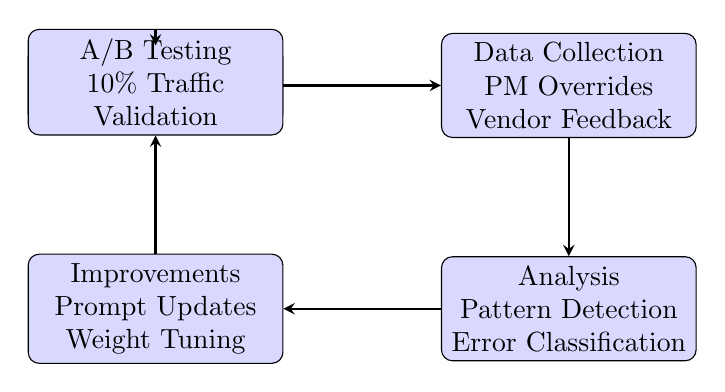
\begin{tikzpicture}[
    node distance=1.5cm and 2cm,
    box/.style={rectangle, draw, fill=blue!15, text width=3cm, align=center, rounded corners, minimum height=1cm},
    arrow/.style={->, >=stealth, thick}
]

\node[box] (production) {Production\\AI System};
\node[box, right=of production] (collect) {Data Collection\\PM Overrides\\Vendor Feedback};
\node[box, below=of collect] (analyze) {Analysis\\Pattern Detection\\Error Classification};
\node[box, left=of analyze] (improve) {Improvements\\Prompt Updates\\Weight Tuning};
\node[box, above=of improve] (test) {A/B Testing\\10\% Traffic\\Validation};

\draw[arrow] (production) -- (collect);
\draw[arrow] (collect) -- (analyze);
\draw[arrow] (analyze) -- (improve);
\draw[arrow] (improve) -- (test);
\draw[arrow] (test) -- (production);

\end{tikzpicture}
\caption{Continuous Learning Feedback Loop}
\end{figure}

\subsubsection{Retraining Cadence}

\begin{table}[H]
\centering
\begin{tabular}{lll}
\toprule
\textbf{Component} & \textbf{Frequency} & \textbf{Trigger} \\
\midrule
Prompt Engineering & Weekly & 50+ new PM overrides \\
Priority Weights & Monthly & SLA breach rate >5\% \\
Model Fine-tuning & Quarterly & 500+ labeled corrections \\
Safety Rules & As needed & Any emergency miss \\
\bottomrule
\end{tabular}
\caption{Retraining Schedule}
\end{table}

 

% ============================================================================
% DEPLOYMENT STRATEGY
% ============================================================================



 



% ============================================================================
% APPENDICES
% ============================================================================
\section{Appendices}

\subsection{Appendix A: Example Classifications}

\subsubsection{Example 1: EMERGENCY with Health Symptoms}

\begin{tcolorbox}[colback=red!5!white,colframe=red!75!black,title=Example EMERGENCY Case]

\textbf{Input:}
\begin{itemize}[itemsep=0pt]
    \item Description: "Gas smell in basement, very strong, making us dizzy, evacuated to neighbor"
    \item Category: HVAC
    \item Images: None
    \item Time: 11:30 PM Sunday
    \item Tenant: Family with infant
    \item Weather: 28°F, winter
\end{itemize}

\textbf{Safety Net:} Catches "gas smell" → EMERGENCY, score=100

\textbf{Agent 1 Output:}
\begin{lstlisting}[language=json, basicstyle=\ttfamily\scriptsize]
{
    "severity": "EMERGENCY",
    "trade": "HVAC",
    "reasoning": "Gas leak with health symptoms (dizziness) and evacuation. Life-safety emergency requiring immediate response per protocol.",
    "confidence": 1.0,
    "key_factors": ["gas_leak", "health_symptoms", "evacuation"]
}
\end{lstlisting}

\textbf{Agent 2 Output:}
\begin{lstlisting}[language=json, basicstyle=\ttfamily\scriptsize]
{
    "priority_score": 100,
    "base_score": 85,
    "applied_modifiers": [
        {"category": "safety", "points": 20, "reason": "gas leak"},
        {"category": "health", "points": 12, "reason": "health symptoms"},
        {"category": "tenant_impact", "points": 10, "reason": "infant present"},
        {"category": "time", "points": 7, "reason": "late night"}
    ],
    "total_modifiers": 49,
    "capped_at": 100
}
\end{lstlisting}

\textbf{Agent 3 Output:}
\begin{lstlisting}[language=json, basicstyle=\ttfamily\scriptsize]
{
    "pm_explanation": "EMERGENCY: Gas leak with evacuation is life-safety emergency. Health symptoms indicate dangerous exposure. Requires immediate emergency vendor dispatch.",
    "tenant_explanation": "Your request has been marked as an emergency. An emergency technician will contact you within 30 minutes. Please stay evacuated until confirmed safe."
}
\end{lstlisting}

\textbf{Agent 4 Output:}
\begin{lstlisting}[language=json, basicstyle=\ttfamily\scriptsize]
{
    "confidence": 1.0,
    "routing": "AUTO_APPROVE_EMERGENCY"
}
\end{lstlisting}

\textbf{Agent 5 Output:}
\begin{lstlisting}[language=json, basicstyle=\ttfamily\scriptsize]
{
    "tier": "EMERGENCY",
    "response_deadline": "2024-12-08 12:00 AM",  # 30 minutes
    "resolution_deadline": "2024-12-08 11:30 PM"  # 24 hours
}
\end{lstlisting}

\textbf{Result:} Auto-approved, emergency vendor dispatched immediately, PM notified

\end{tcolorbox}

 

\subsubsection{Example 2: HIGH with Active Water Damage}

\begin{tcolorbox}[colback=yellow!5!white,colframe=yellow!75!black,title=Example HIGH Case]

\textbf{Input:}
\begin{itemize}[itemsep=0pt]
    \item Description: "Toilet overflowing, water spreading to bedroom, can't stop it"
    \item Category: PLUMBING
    \item Images: 2 photos showing water on floor
    \item Time: 10:00 PM Saturday
    \item Tenant: Elderly (78 years old)
    \item Weather: Normal
\end{itemize}

\textbf{Safety Net:} No emergency keywords detected, continue to AI

\textbf{Agent 1 Output:}
\begin{lstlisting}[language=json, basicstyle=\ttfamily\scriptsize]
{
    "severity": "HIGH",
    "trade": "PLUMBING",
    "reasoning": "Active overflow with water spreading beyond bathroom. Property damage occurring and toilet is essential service. Elderly tenant increases urgency.",
    "confidence": 0.95,
    "key_factors": ["active_water_damage", "spreading", "essential_service_loss"]
}
\end{lstlisting}

\textbf{Agent 2 Output:}
\begin{lstlisting}[language=json, basicstyle=\ttfamily\scriptsize]
{
    "priority_score": 78,
    "base_score": 60,
    "applied_modifiers": [
        {"category": "water_damage", "points": 15, "reason": "spreading water"},
        {"category": "tenant_impact", "points": 8, "reason": "elderly"},
        {"category": "essential_service", "points": 12, "reason": "toilet unusable"},
        {"category": "time", "points": 6, "reason": "weekend after hours"}
    ],
    "total_modifiers": 41,
    "capped_at": 84  # MAX for HIGH
}
\end{lstlisting}

\textbf{Agent 3 Output:}
\begin{lstlisting}[language=json, basicstyle=\ttfamily\scriptsize]
{
    "pm_explanation": "Active overflow with water spreading requires urgent response to prevent property damage. Loss of toilet function with elderly tenant. Recommend same-day emergency plumber.",
    "tenant_explanation": "We understand this is urgent. An emergency plumber will contact you within 2 hours to schedule an immediate visit today."
}
\end{lstlisting}

\textbf{Agent 4 Output:}
\begin{lstlisting}[language=json, basicstyle=\ttfamily\scriptsize]
{
    "confidence": 0.95,
    "routing": "AUTO_APPROVE"
}
\end{lstlisting}

\textbf{Agent 5 Output:}
\begin{lstlisting}[language=json, basicstyle=\ttfamily\scriptsize]
{
    "tier": "HIGH",
    "response_deadline": "2024-12-08 12:00 PM",  # Next day noon
    "resolution_deadline": "2024-12-09 10:00 PM"  # 48 hours
}
\end{lstlisting}

\textbf{Result:} Auto-approved, emergency plumber assigned same-day

\end{tcolorbox}

 

\subsubsection{Example 3: MEDIUM with Seasonal Context}

\begin{tcolorbox}[colback=blue!5!white,colframe=blue!75!black,title=Example MEDIUM Case]

\textbf{Input:}
\begin{itemize}[itemsep=0pt]
    \item Description: "Water heater making loud banging noises, sounds weird, 15 year old unit"
    \item Category: PLUMBING
    \item Images: None
    \item Time: 2:00 PM Wednesday
    \item Tenant: Standard (no vulnerabilities)
    \item Weather: 32°F, winter
\end{itemize}

\textbf{Safety Net:} No emergency keywords, continue to AI

\textbf{Agent 1 Output:}
\begin{lstlisting}[language=json, basicstyle=\ttfamily\scriptsize]
{
    "severity": "MEDIUM",
    "trade": "PLUMBING",
    "reasoning": "Unusual noise from aging water heater suggests mineral buildup or thermal expansion. Not immediately dangerous but should be inspected within 24-48 hours to prevent failure. Winter season increases priority.",
    "confidence": 0.88,
    "key_factors": ["unusual_noise", "unit_age_15yr", "winter_season"]
}
\end{lstlisting}

\textbf{Agent 2 Output:}
\begin{lstlisting}[language=json, basicstyle=\ttfamily\scriptsize]
{
    "priority_score": 48,
    "base_score": 30,
    "applied_modifiers": [
        {"category": "seasonal", "points": 8, "reason": "winter, no hot water risk"},
        {"category": "property_risk", "points": 10, "reason": "aging unit may fail"}
    ],
    "total_modifiers": 18,
    "capped_at": null
}
\end{lstlisting}

\textbf{Agent 3 Output:}
\begin{lstlisting}[language=json, basicstyle=\ttfamily\scriptsize]
{
    "pm_explanation": "Loud banging from 15-year water heater indicates potential failure risk. MEDIUM priority requires 24-48 hour inspection to prevent winter hot water loss.",
    "tenant_explanation": "We'll have a plumber inspect your water heater within 1-2 business days. The noise suggests it needs maintenance to prevent issues."
}
\end{lstlisting}

\textbf{Agent 4 Output:}
\begin{lstlisting}[language=json, basicstyle=\ttfamily\scriptsize]
{
    "confidence": 0.88,
    "routing": "AUTO_APPROVE"
}
\end{lstlisting}

\textbf{Agent 5 Output:}
\begin{lstlisting}[language=json, basicstyle=\ttfamily\scriptsize]
{
    "tier": "MEDIUM",
    "response_deadline": "2024-12-09 6:00 PM",  # 48 business hours
    "resolution_deadline": "2024-12-12 6:00 PM"  # 5 business days
}
\end{lstlisting}

\textbf{Result:} Auto-approved, standard plumber assigned within 48 hours

\end{tcolorbox}

 

\subsection{Appendix B: Glossary}

\begin{description}
    \item[Agent] A specialized LLM model with a specific task (e.g., Triage Classifier, Priority Calculator)
    
    \item[Confidence Score] A value from 0.0 to 1.0 indicating the AI's certainty in its classification
    
    \item[Context Bundle] A JSON object containing all enriched contextual data (weather, tenant, property, history)
    
    \item[Emergency] Highest severity level (85-100 priority score) requiring immediate response for life-safety issues
    
    \item[Multimodal] LLM capability to process both text and images simultaneously
    
    \item[PM] Property Manager - the human decision-maker who reviews and approves AI classifications
    
    \item[Priority Score] Numerical urgency index from 0-100 combining severity and contextual modifiers
    
    \item[Safety Net] Deterministic rules engine that catches life-threatening emergencies before AI processing
    
    \item[SLA] Service Level Agreement - contractual response and resolution timeframes
    
    \item[Trade] Category of repair work (PLUMBING, ELECTRICAL, HVAC, APPLIANCE, GENERAL, STRUCTURAL)
    
    \item[Triage] The process of classifying maintenance requests by severity and urgency
    
    \item[Vector Search] Similarity search using embeddings to find past cases matching the current request
\end{description}

\subsection{Appendix C: Revision History}

\begin{table}[H]
\centering
\begin{tabular}{lllp{5cm}}
\toprule
\textbf{Version} & \textbf{Date} & \textbf{Author} & \textbf{Changes} \\
\midrule
1.0 & 2024-12-07 & Engineering Team & Initial release - Complete architecture specification \\
\bottomrule
\end{tabular}
\caption{Document Revision History}
\end{table}

 

% ============================================================================
% CONCLUSION
% ============================================================================



\end{document}